
\documentclass{beamer}

\usetheme{PSY9511}

\usepackage{pgfplots}
\usepackage{pgfplotstable}
\usepackage{tikz}

\usepgfplotslibrary{fillbetween}
\usepgfplotslibrary{groupplots}

\usetikzlibrary{arrows.meta}
\usetikzlibrary{calc}

\title{Explainable AI and the brain}
\subtitle{Characterizing heterogeneity in diverse clinical cohorts}
\author{Esten H. Leonardsen}
\date{24.10.24}

\begin{document}
	\begin{frame}
	 	\maketitle
	\end{frame}

    \begin{frame}{Outline}
        \begin{enumerate}
            \item Theoretical background
            \begin{enumerate}
                \item[a.] Artificial neural networks
                \item[b.] Explainable AI
            \end{enumerate}
            \item Explainable AI and dementia
            \item Explainable AI and brain age
        \end{enumerate}
    \end{frame}

    \newcommand{\mriside}[4]{
    \def\mridepth{0.75}

    \node[inner sep=0pt] (input) at (#1, #2) {
        \includegraphics[height=#3, width=#3]{#4}
    };

    \draw[fill=black] (input.north west) --
        ($ (input.north west) + (0.5 * \mridepth, 0.5 * \mridepth) $) --
        ($ (input.north east) + (0.5 * \mridepth, 0.5 * \mridepth) $) --
        (input.north east) -- cycle;
    \draw[fill=black] (input.north east) --
        ($ (input.north east) + (0.5 * \mridepth, 0.5 * \mridepth) $) --
        ($ (input.south east) + (0.5 * \mridepth, 0.5 * \mridepth) $) --
        (input.south east) -- cycle;
    \draw[] (input.north west) --
        ($ (input.north west) - (0.5 * \mridepth, 0.5 * \mridepth) $) --
        ($ (input.south west) - (0.5 * \mridepth, 0.5 * \mridepth) $) --
        (input.south west) -- cycle;
    \draw[] (input.north east) --
        ($ (input.north east) - (0.5 * \mridepth, 0.5 * \mridepth) $) --
        ($ (input.south east) - (0.5 * \mridepth, 0.5 * \mridepth) $) --
        (input.south east) -- cycle;
    \draw[] ($ (input.north west) - (0.5 * \mridepth, 0.5 * \mridepth) $) --
        ($ (input.north east) - (0.5 * \mridepth, 0.5 * \mridepth) $);
    \draw[] ($ (input.south west) - (0.5 * \mridepth, 0.5 * \mridepth) $) --
        ($ (input.south east) - (0.5 * \mridepth, 0.5 * \mridepth) $);
}


\newcommand{\inputside}[3]{
    \mriside{#1}{#2}{#3}{data/mri_sagittal.png}
}

\newcommand{\heatmapside}[3]{
    \mriside{#1}{#2}{#3}{data/combined_sagittal.png}
}

\newcommand{\convside}[6]{
    \def\sidex{#1}
    \def\sidey{#2}
    \def\sidewidth{#3}
    \def\sideheight{#4}
    \def\sidefillcolour{#5}
    \def\sidename{#6}

    \node[
        fill=\sidefillcolour,
        inner sep=0pt,
        outer sep=0pt,
        minimum width=\sidewidth,
        minimum height=\sideheight,
        draw=black
    ] (\sidename) at (\sidex, \sidey) {};
}

\newcommand{\convtop}[4]{
    \def\topbase{#1}
    \def\topwidth{#2}
    \def\topheight{#3}
    \def\topfillcolour{#4}

    \draw[fill=\topfillcolour,draw=black] #1 --
        ($ #1 + (#3, #3) $) --
        ($ #1 + (#3+#2, #3) $) --
        ($ #1 + (#2, 0) $);
}

\newcommand{\convfront}[3]{
    \def\frontbase{#1}
    \def\frontsize{#2}
    \def\frontfillcolour{#3}

    \draw[black, fill=\frontfillcolour] #1 --
        ($ #1 + (1*#2, 1*#2) $) --
        ($ #1 + (1*#2, 1*#2 - 2*#2) $) --
        ($ #1 + (0, -2*#2) $);
}

\newcommand{\convchannel}[7]{
    \def\channelx{#1}
    \def\channely{#2}
    \def\channelnodedepth{#3}
    \def\channelnodesize{#4}
    \def\channelnodecount{#5}
    \def\channelcolour{#6}
    \def\includefront{#7}

    \def\huemin{20}
    \def\huemax{80}

    \pgfmathsetmacro{\iterations}{#5-1}
    \foreach \i in {0,...,\iterations} {
        \pgfmathsetmacro{\hue}{int(random(\huemin, \huemax))}
        \convside{#1}{#2+\i*-#4}{#3 cm}{#4 cm}{#6!\hue}{n\i0}

        \foreach \j in {0,...,\iterations} {
            \pgfmathsetmacro{\innerhue}{int(random(\huemin, \huemax))}
            \ifnum\j=0
                \pgfmathsetmacro{\innerhue}{\hue}
            \fi

            \ifnum\includefront=1
                \convfront{($ (n00.north east) + (0.5*\j*#4, 0.5*\j*#4 - \i*#4) $)}{0.5*#4}{#6!\innerhue}
            \fi

            \ifnum\i=0
                \convtop{($ (n\i0.north west) + (0.5*\j*#4, 0.5*\j*#4) $)}{#3}{0.5*#4}{#6!\innerhue}
            \fi
        }
    }
}
\newcommand{\lrpchannel}[6]{
    \def\channelx{#1}
    \def\channely{#2}
    \def\channelnodedepth{#3}
    \def\channelnodesize{#4}
    \def\channelnodecount{#5}
    \def\includefront{#6}

    \colorlet{bgcolour}{black!85}

    \pgfmathsetmacro{\iterations}{#5-1}
    \foreach \i in {0,...,\iterations} {
        \pgfmathsetmacro{\hue}{int(random(-150, 100))}
        \colorlet{fillcolour}{bgcolour}

        \colorlet{lrpcolour}{red}
        \pgfmathsetmacro{\coinflip}{int(random(0, 1))}

        \ifnum\coinflip=1
            \colorlet{lrpcolour}{blue}
        \fi

        \ifnum\hue>0
            \colorlet{fillcolour}{lrpcolour!\hue!bgcolour}
        \fi

        \convside{#1}{#2+\i*-#4}{#3 cm}{#4 cm}{fillcolour}{n\i0}

        \foreach \j in {0,...,\iterations} {
            \pgfmathsetmacro{\innerhue}{int(random(-150, 100))}
            \colorlet{innerfillcolour}{bgcolour}

            \ifnum\innerhue>0
                \colorlet{innerfillcolour}{lrpcolour!\innerhue!bgcolour}
            \fi

            \ifnum\j=0
                \colorlet{innerfillcolour}{fillcolour}
            \fi

            \ifnum\includefront=1
                \convfront{($ (n00.north east) + (0.5*\j*#4, 0.5*\j*#4 - \i*#4) $)}{0.5*#4}{innerfillcolour}
            \fi

            \ifnum\i=0
                \convtop{($ (n\i0.north west) + (0.5*\j*#4, 0.5*\j*#4) $)}{#3}{0.5*#4}{innerfillcolour}
            \fi
        }
    }
}


\newcommand{\convlayer}[7]{
    \def\layerx{#1}
    \def\layery{#2}
    \def\layernodedepth{#3}
    \def\layernodesize{#4}
    \def\layernodecount{#5}
    \def\layerdepth{#6}
    \def\layercolour{#7}

    \pgfmathsetmacro{\layeriterations}{\layerdepth-1}
    \foreach \i in {0,...,\layeriterations}{
        \pgfmathsetmacro{\x}{\layerx + \i * \layernodedepth}
        \pgfmathsetmacro{\islast}{\i == \layeriterations ? 1 : 0}
        \convchannel{\x}{\layery}{\layernodedepth}{\layernodesize}{\layernodecount}{\layercolour}{\islast}
    }
}
\newcommand{\lrplayer}[6]{
    \def\layerx{#1}
    \def\layery{#2}
    \def\layernodedepth{#3}
    \def\layernodesize{#4}
    \def\layernodecount{#5}
    \def\layerdepth{#6}

    \pgfmathsetmacro{\layeriterations}{\layerdepth-1}
    \foreach \i in {0,...,\layeriterations}{
        \pgfmathsetmacro{\x}{\layerx + \i * \layernodedepth}
        \pgfmathsetmacro{\islast}{\i == \layeriterations ? 1 : 0}
        \lrpchannel{\x}{\layery}{\layernodedepth}{\layernodesize}{\layernodecount}{\islast}
    }
}

\newcommand{\modelarrow}[5]{
    \begin{scope}[transparency group, opacity=0.5]
        \draw[-stealth, line width=2pt, #3] #1 to [in=#4, out=#5] #2;
    \end{scope}
}
\newcommand{\cnnarrow}[3]{
    \modelarrow{#1}{#2}{#3}{180}{0}
}
\newcommand{\lrparrow}[3]{
    \modelarrow{#1}{#2}{#3}{0}{180}
}

\newcommand{\cnn}[6]{
    \def\xmin{#1}
    \def\ymin{#2}
    \def\nodedepth{#3}
    \def\nodesize{#4}
    \def\modelcolour{#5}
    \def\annotate{#6}

    \convlayer{#1 - 0.06 + 0.4}{#2 + 2.5 * #4}{#3}{#4}{12}{3}{\modelcolour}
    \cnnarrow{(#1 + 1.04, #2)}{(#1+2.2, #2)}{black}

    \convlayer{#1 + 1.44 + 0.4}{#2 + 1.5 * #4}{#3}{#4}{8}{5}{\modelcolour}
    \cnnarrow{(#1 + 2.59, #2)}{(#1+3.5, #2)}{black}

    \convlayer{#1 + 2.77 + 0.4}{#2 + 0.5 * #4}{#3}{#4}{4}{7}{\modelcolour}
    \cnnarrow{(#1 + 3.98, #2)}{(#1+5, #2)}{black}

    \convlayer{#1 + 3.93 + 0.4}{#2 + 0}{#3}{#4}{2}{9}{\modelcolour}

    \draw[thick, dashed] (#1 + 0.22, #2 + 1.43) --
                        (#1 + 5.4, #2 + 1.43) --
                        (#1 + 5.4, #2 - 1.42) --
                        (#1 + 0.22, #2 - 1.42) -- cycle;
    \node[anchor=south, text depth=0, font=\footnotesize\selectfont] at (#1 + 2.675, #2 + 1.43) {
        \textbf{Convolutional neural network}
    };
}
\newcommand{\lrp}[4]{
    \def\xmin{#1}
    \def\ymin{#2}
    \def\nodedepth{#3}
    \def\nodesize{#4}

    \lrplayer{#1 - 0.06 + 0.4}{#2 + 2.5 * #4}{#3}{#4}{12}{3}{black}
    \lrparrow{(#1+2.2, #2)}{(#1 + 1.04, #2)}{black}

    \lrplayer{#1 + 1.44 + 0.4}{#2 + 1.5 * #4}{#3}{#4}{8}{5}{black}
    \lrparrow{(#1+3.5, #2)}{(#1 + 2.59, #2)}{black}

    \lrplayer{#1 + 2.77 + 0.4}{#2 + 0.5 * #4}{#3}{#4}{4}{7}{black}
    \lrparrow{(#1+5, #2)}{(#1 + 3.98, #2)}{black}

    \lrplayer{#1 + 3.93 + 0.4}{#2 + 0}{#3}{#4}{2}{9}{black}

    \draw[thick, dashed] (#1 + 0.22, #2 + 1.43) --
                        (#1 + 5.4, #2 + 1.43) --
                        (#1 + 5.4, #2 - 1.42) --
                        (#1 + 0.22, #2 - 1.42) -- cycle;
    \node[anchor=south, text depth=0, font=\footnotesize\selectfont] at (#1 + 2.675, #2 + 1.43) {
        \textbf{Convolutional Neural Network}
    };
}
    \newcommand{\datapoints}[1]{
    \begin{tikzpicture}
        \begin{axis}[
            height=3.5cm,
            width=6cm,
            xmajorticks=false,
            ymajorticks=false,
            xmin=-7,
            xmax=7,
            xlabel=\footnotesize{\textbf{x}},
            ylabel=\footnotesize{\textbf{y}}
        ]
            \addplot[
                only marks,
                blue,
                opacity=0.5,
                samples=50,
                domain=-7:7
            ] {x^3 - 3*x^2 + 2*x + 150 * rand};
            \addplot[
                red,
                domain=-7:7,
                thick
            ] {40*x-50};

            \ifnum#1>0
                \addplot[
                    green,
                    domain=-7:7,
                    thick
                ] {x^3 - 3*x^2 + 2*x};
                \node[anchor=south east, font=\tiny, align=left] (legend) at (rel axis cs: 1, 0) {
                    Linear Regression Model\\
                    Artificial Neural Network
                };
                \draw[red, thick] (rel axis cs: 0.43, 0.25) -- (rel axis cs: 0.38, 0.25);
                \draw[green, thick] (rel axis cs: 0.43, 0.11) -- (rel axis cs: 0.38, 0.11);

            \fi
        \end{axis}
    \end{tikzpicture}
}

\newcommand{\neuron}[3]{
    \node[circle, draw=black, fill=#2] (#1) at #3 {};
}

\begin{frame}{Artificial neural networks}
    \begin{tikzpicture}
        \node[draw=black] at (-5.25, -3.25) {};
        \node[draw=black] at (5.25, 3.25) {};

        \only<1-6>{
            \node[
                draw=black,
                fill=cyan!15,
                minimum height=3cm,
                minimum width=4.3cm
            ] (model) at (0, 1) {
                \only<2-3>{$y=\beta_0+\beta_1x$}
            };
        }
        \only<1-5>{
            \node[] (input) at ($ (model.west) + (-1, 0) $) {$\mathbf{x}$};
            \draw[-Latex] (input) -- (model);

            \node[] (output) at ($ (model.east) + (1, 0) $) {$\mathbf{y}$};
            \draw[-Latex] (model) -- (output);
        }
        \only<1>{
            \node[font=\footnotesize] (inputlabel) at ($ (input.south) - (0, 0.5) $) {Input};
            \draw[-stealth, gray] (inputlabel) -- (input);

            \node[font=\footnotesize] (outputlabel) at ($ (output.south) - (0, 0.5) $) {Output};
            \draw[-stealth, gray] (outputlabel) -- (output);

            \node[
                anchor=south,
                font=\small
            ] at (model.north) {Predictive model};
        }
        \only<2-3>{
            \node[
                anchor=south,
                font=\small
            ] at (model.north) {Linear regression model};
        }
        \visible<3>{
            \node[] at (-0.15, -2.2) {
                \datapoints{0}
            };
        }
        \only<4-6>{
            \node[
                anchor=south,
                font=\small
            ] at (model.north) {Artificial neural network};

            \def\hsep{0.7}
            \def\vsep{0.5}
            \def\edgecolor{gray}
            \def\edgeopacity{0.5}
            \def\neuroncolour{gray}

            \neuron{n00}{\neuroncolour}{($ (model) + (-2 * \hsep, -2 * \vsep) $)}
            \neuron{n01}{\neuroncolour}{($ (model) + (-2 * \hsep, -\vsep) $)}
            \neuron{n02}{\neuroncolour}{($ (model) + (-2 * \hsep, 0) $)}
            \neuron{n03}{\neuroncolour}{($ (model) + (-2 * \hsep, \vsep) $)}
            \neuron{n04}{\neuroncolour}{($ (model) + (-2 * \hsep, 2 * \vsep) $)}

            \neuron{n10}{\neuroncolour}{($ (model) + (-\hsep, -1.5 * \vsep) $)}
            \neuron{n11}{\neuroncolour}{($ (model) + (-\hsep, -0.5 * \vsep) $)}
            \neuron{n12}{\neuroncolour}{($ (model) + (-\hsep, 0.5 * \vsep) $)}
            \neuron{n13}{\neuroncolour}{($ (model) + (-\hsep, 1.5 * \vsep) $)}

            \neuron{n20}{\neuroncolour}{($ (model) + (0, -\vsep) $)}
            \neuron{n21}{\neuroncolour}{(model)}
            \neuron{n22}{\neuroncolour}{($ (model) + (0, \vsep) $)}

            \neuron{n30}{\neuroncolour}{($ (model) + (\hsep, -0.5 * \vsep) $)}
            \neuron{n31}{\neuroncolour}{($ (model) + (\hsep, 0.5 * \vsep) $)}

            \neuron{n40}{\neuroncolour}{($ (model) + (2 * \hsep, 0) $)}

            \draw[-stealth, \edgecolor, opacity=\edgeopacity] (model.west) -- (n00);
            \draw[-stealth, \edgecolor, opacity=\edgeopacity] (model.west) -- (n01);
            \draw[-stealth, \edgecolor, opacity=\edgeopacity] (model.west) -- (n02);
            \draw[-stealth, \edgecolor, opacity=\edgeopacity] (model.west) -- (n03);
            \draw[-stealth, \edgecolor, opacity=\edgeopacity] (model.west) -- (n04);

            \foreach \i in {0,...,4} {
                \foreach \j in {0,...,3} {
                    \draw[\edgecolor, opacity=\edgeopacity] (n0\i) -- (n1\j);
                }
            }
            \foreach \i in {0,...,3} {
                \foreach \j in {0,...,2} {
                    \draw[\edgecolor, opacity=\edgeopacity] (n1\i) -- (n2\j);
                }
            }
            \foreach \i in {0,...,2} {
                \foreach \j in {0,...,1} {
                    \draw[\edgecolor, opacity=\edgeopacity] (n2\i) -- (n3\j);
                }
            }
            \foreach \i in {0,...,1} {
                \draw[\edgecolor, opacity=\edgeopacity] (n3\i) -- (n40);
            }

            \draw[-stealth, \edgecolor, opacity=\edgeopacity] (n40) -- (model.east);
        }
        \visible<5>{
            \node[] at (-0.15, -2.2) {
                \datapoints{1}
            };
        }
        \visible<6>{
            \node[anchor=east, draw=black, inner sep=0pt, outer sep=3pt] (input) at ($ (model.west) + (-0.77, 0) $) {
                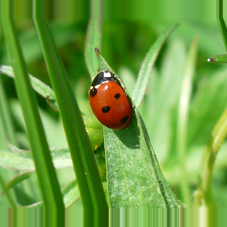
\includegraphics[width=2cm]{data/ladybug.png}
            };
            \draw[-Latex] (input) -- (model);

            \node[anchor=west] (output) at ($ (model.east) + (0.77, 0) $) {
                ladybug
            };
            \draw[-Latex] (model) -- (output);
        }
    \end{tikzpicture}
\end{frame}

\begin{frame}{Artificial neural networks: Interpretability}
    \begin{tikzpicture}
        \node[draw=black] at (-5.25, -3.25) {};
        \node[draw=black] at (5.25, 3.25) {};

        \node[
            draw=black,
            fill=cyan!15,
            minimum height=3cm,
            minimum width=4.3cm
        ] (model) at (0, 1) {};
        \node[
            anchor=south,
            font=\small
        ] at (model.north) {Artificial neural network};

        \only<1-4>{
            \node[] (input) at ($ (model.west) + (-1, 0) $) {$\mathbf{x}$};
            \draw[-Latex] (input) -- (model);
        }
        \only<1-10>{
            \node[] (output) at ($ (model.east) + (1, 0) $) {$\mathbf{y}$};
            \draw[-Latex] (model) -- (output);
        }
        \only<1,3->{
            \node[
                anchor=south,
                font=\small
            ] at (model.north) {Artificial neural network};

            \def\hsep{0.7}
            \def\vsep{0.5}
            \def\edgecolor{gray}
            \def\edgeopacity{0.5}
            \def\neuroncolour{gray}

            \only<1-5>{
                \neuron{n00}{\neuroncolour}{($ (model) + (-2 * \hsep, -2 * \vsep) $)}
                \neuron{n01}{\neuroncolour}{($ (model) + (-2 * \hsep, -\vsep) $)}
                \neuron{n02}{\neuroncolour}{($ (model) + (-2 * \hsep, 0) $)}
                \neuron{n03}{\neuroncolour}{($ (model) + (-2 * \hsep, \vsep) $)}
                \neuron{n04}{\neuroncolour}{($ (model) + (-2 * \hsep, 2 * \vsep) $)}
            }
            \only<6->{
                \neuron{n00}{black!25}{($ (model) + (-2 * \hsep, -2 * \vsep) $)}
                \neuron{n01}{black!90}{($ (model) + (-2 * \hsep, -\vsep) $)}
                \neuron{n02}{black!72}{($ (model) + (-2 * \hsep, 0) $)}
                \neuron{n03}{black!99}{($ (model) + (-2 * \hsep, \vsep) $)}
                \neuron{n04}{black!10}{($ (model) + (-2 * \hsep, 2 * \vsep) $)}
            }

            \only<1-6>{
                \neuron{n10}{\neuroncolour}{($ (model) + (-\hsep, -1.5 * \vsep) $)}
                \neuron{n11}{\neuroncolour}{($ (model) + (-\hsep, -0.5 * \vsep) $)}
                \neuron{n12}{\neuroncolour}{($ (model) + (-\hsep, 0.5 * \vsep) $)}
                \neuron{n13}{\neuroncolour}{($ (model) + (-\hsep, 1.5 * \vsep) $)}
            }
            \only<7->{
                \neuron{n10}{black!55}{($ (model) + (-\hsep, -1.5 * \vsep) $)}
                \neuron{n11}{black!92}{($ (model) + (-\hsep, -0.5 * \vsep) $)}
                \neuron{n12}{black!31}{($ (model) + (-\hsep, 0.5 * \vsep) $)}
                \neuron{n13}{black!7}{($ (model) + (-\hsep, 1.5 * \vsep) $)}
            }
            \only<1-7>{
                \neuron{n20}{\neuroncolour}{($ (model) + (0, -\vsep) $)}
                \neuron{n21}{\neuroncolour}{(model)}
                \neuron{n22}{\neuroncolour}{($ (model) + (0, \vsep) $)}
            }
            \only<8->{
                \neuron{n20}{black!50}{($ (model) + (0, -\vsep) $)}
                \neuron{n21}{black!10}{(model)}
                \neuron{n22}{black!100}{($ (model) + (0, \vsep) $)}
            }

            \only<1-8>{
                \neuron{n30}{\neuroncolour}{($ (model) + (\hsep, -0.5 * \vsep) $)}
                \neuron{n31}{\neuroncolour}{($ (model) + (\hsep, 0.5 * \vsep) $)}
            }
            \only<9->{
                \neuron{n30}{black!75}{($ (model) + (\hsep, -0.5 * \vsep) $)}
                \neuron{n31}{black!65}{($ (model) + (\hsep, 0.5 * \vsep) $)}
            }
            \only<1-9>{
                \neuron{n40}{\neuroncolour}{($ (model) + (2 * \hsep, 0) $)}
            }
            \only<10->{
                \neuron{n40}{black!95}{($ (model) + (2 * \hsep, 0) $)}
            }

            \only<1-5,7->{
                \draw[-stealth, \edgecolor, opacity=\edgeopacity] (model.west) -- (n00);
                \draw[-stealth, \edgecolor, opacity=\edgeopacity] (model.west) -- (n01);
                \draw[-stealth, \edgecolor, opacity=\edgeopacity] (model.west) -- (n02);
                \draw[-stealth, \edgecolor, opacity=\edgeopacity] (model.west) -- (n03);
                \draw[-stealth, \edgecolor, opacity=\edgeopacity] (model.west) -- (n04);
            }
            \only<6>{
                \draw[-stealth, red, opacity=\edgeopacity] (model.west) -- (n00);
                \draw[-stealth, red, opacity=\edgeopacity] (model.west) -- (n01);
                \draw[-stealth, red, opacity=\edgeopacity] (model.west) -- (n02);
                \draw[-stealth, red, opacity=\edgeopacity] (model.west) -- (n03);
                \draw[-stealth, red, opacity=\edgeopacity] (model.west) -- (n04);
            }

            \only<1-6,8->{
                \foreach \i in {0,...,4} {
                    \foreach \j in {0,...,3} {
                        \draw[\edgecolor, opacity=\edgeopacity] (n0\i) -- (n1\j);
                    }
                }
            }
            \only<7>{
                \foreach \i in {0,...,4} {
                    \foreach \j in {0,...,3} {
                        \draw[red, opacity=\edgeopacity] (n0\i) -- (n1\j);
                    }
                }
            }

            \only<1-7,9->{
                \foreach \i in {0,...,3} {
                    \foreach \j in {0,...,2} {
                        \draw[\edgecolor, opacity=\edgeopacity] (n1\i) -- (n2\j);
                    }
                }
            }
            \only<8>{
                \foreach \i in {0,...,3} {
                    \foreach \j in {0,...,2} {
                        \draw[red, opacity=\edgeopacity] (n1\i) -- (n2\j);
                    }
                }
            }

            \only<1-8,10->{
                \foreach \i in {0,...,2} {
                    \foreach \j in {0,...,1} {
                        \draw[\edgecolor, opacity=\edgeopacity] (n2\i) -- (n3\j);
                    }
                }
            }
            \only<9>{
                \foreach \i in {0,...,2} {
                    \foreach \j in {0,...,1} {
                        \draw[red, opacity=\edgeopacity] (n2\i) -- (n3\j);
                    }
                }
            }
            \only<1-9,11->{
                \foreach \i in {0,...,1} {
                    \draw[\edgecolor, opacity=\edgeopacity] (n3\i) -- (n40);
                }
            }
            \only<10>{
                \foreach \i in {0,...,1} {
                    \draw[red, opacity=\edgeopacity] (n3\i) -- (n40);
                }
            }

            \only<1-10,12-13>{
                \draw[-stealth, \edgecolor, opacity=\edgeopacity] (n40) -- (model.east);
            }
            \only<11>{
                \draw[-stealth, red, opacity=\edgeopacity] (n40) -- (model.east);
            }
        }
        \only<2>{
            \node[
                draw=black,
                fill=black,
                minimum height=3cm,
                minimum width=4.3cm
            ] (model) at (0, 1) {};
        }
        \only<3>{
            \node[] at (-0.15, -2.2) {
                \datapoints{1}
            };
        }
        \only<5-11>{
            \node[] (input) at ($ (model.west) + (-1, 0) $) {$5$};
        }
        \only<5,7-11>{
            \draw[-Latex] (input) -- (model);
        }
        \only<6>{
            \draw[-Latex, red] (input) -- (model);
        }
        \only<11>{
            \node[text=red] (output) at ($ (model.east) + (1, 0) $) {3};
            \draw[-Latex, red] (model) -- (output);
        }
        \only<12-13>{
            \node[anchor=east, draw=black, inner sep=0pt, outer sep=3pt] (input) at ($ (model.west) + (-0.77, 0) $) {
                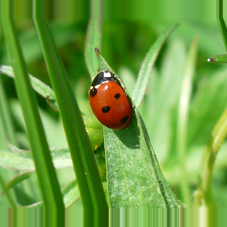
\includegraphics[width=2cm]{data/ladybug.png}
            };
            \draw[-Latex] (input) -- (model);

            \node[anchor=west] (output) at ($ (model.east) + (0.77, 0) $) {
                ladybug
            };
            \draw[-Latex] (model) -- (output);
        }
        \only<13>{
            \node[anchor=north] (pass) at (model.south) {
                \textbf{\textit{Forward pass}}
            };
            \draw[-stealth] (pass.south west) -- (pass.south east);

            \node[] at (0, -2.5) {
                $n^i_j = f(\sum\limits_{k=0}^n w^{i}_{jk} n^{i-1}_k)$
            };
        }
    \end{tikzpicture}
\end{frame}

\begin{frame}{Artificial neural networks: Explainability}
    \begin{tikzpicture}
        \node[draw=black] at (-5.25, -3.25) {};
        \node[draw=black] at (5.25, 3.25) {};

        \node[
            draw=black,
            fill=cyan!15,
            minimum height=3cm,
            minimum width=4.3cm
        ] (model) at (0, 1) {};
        \node[
            anchor=south,
            font=\small
        ] at (model.north) {Artificial neural network};

        \def\hsep{0.7}
        \def\vsep{0.5}
        \def\edgecolor{gray}
        \def\edgeopacity{0.5}
        \def\neuroncolour{gray}

        \neuron{n00}{black!25}{($ (model) + (-2 * \hsep, -2 * \vsep) $)}
        \neuron{n01}{black!90}{($ (model) + (-2 * \hsep, -\vsep) $)}
        \neuron{n02}{black!72}{($ (model) + (-2 * \hsep, 0) $)}
        \neuron{n03}{black!99}{($ (model) + (-2 * \hsep, \vsep) $)}
        \neuron{n04}{black!10}{($ (model) + (-2 * \hsep, 2 * \vsep) $)}

        \neuron{n10}{black!55}{($ (model) + (-\hsep, -1.5 * \vsep) $)}
        \neuron{n11}{black!92}{($ (model) + (-\hsep, -0.5 * \vsep) $)}
        \neuron{n12}{black!31}{($ (model) + (-\hsep, 0.5 * \vsep) $)}
        \neuron{n13}{black!7}{($ (model) + (-\hsep, 1.5 * \vsep) $)}

        \neuron{n20}{black!50}{($ (model) + (0, -\vsep) $)}
        \neuron{n21}{black!10}{(model)}
        \neuron{n22}{black!100}{($ (model) + (0, \vsep) $)}

        \neuron{n30}{black!75}{($ (model) + (\hsep, -0.5 * \vsep) $)}
        \neuron{n31}{black!65}{($ (model) + (\hsep, 0.5 * \vsep) $)}

        \only<1-2>{
            \neuron{n40}{black!95}{($ (model) + (2 * \hsep, 0) $)}
        }
        \only<3>{
            \neuron{n40}{red}{($ (model) + (2 * \hsep, 0) $)}
        }

        \draw[-stealth, \edgecolor, opacity=\edgeopacity] (model.west) -- (n00);
        \draw[-stealth, \edgecolor, opacity=\edgeopacity] (model.west) -- (n01);
        \draw[-stealth, \edgecolor, opacity=\edgeopacity] (model.west) -- (n02);
        \draw[-stealth, \edgecolor, opacity=\edgeopacity] (model.west) -- (n03);
        \draw[-stealth, \edgecolor, opacity=\edgeopacity] (model.west) -- (n04);

        \foreach \i in {0,...,4} {
            \foreach \j in {0,...,3} {
                \draw[\edgecolor, opacity=\edgeopacity] (n0\i) -- (n1\j);
            }
        }

        \foreach \i in {0,...,3} {
            \foreach \j in {0,...,2} {
                \draw[\edgecolor, opacity=\edgeopacity] (n1\i) -- (n2\j);
            }
        }

        \foreach \i in {0,...,2} {
            \foreach \j in {0,...,1} {
                \draw[\edgecolor, opacity=\edgeopacity] (n2\i) -- (n3\j);
            }
        }

        \foreach \i in {0,...,1} {
            \draw[\edgecolor, opacity=\edgeopacity] (n3\i) -- (n40);
        }

        \only<1-2>{
            \draw[-stealth, \edgecolor, opacity=\edgeopacity] (n40) -- (model.east);
        }
        \only<3>{
            \draw[stealth-, red, opacity=\edgeopacity] (n40) -- (model.east);
        }

        \only<1>{
            \node[anchor=north] (pass) at (model.south) {
                \textbf{\textit{Forward pass}}
            };
            \draw[-stealth] (pass.south west) -- (pass.south east);

            \node[] at (0, -2.5) {
                $n^i_j = f(\sum\limits_{k} w^{i}_{jk} n^{(i-1)}_k)$
            };
        }
        \only<1-3>{
            \node[anchor=east, draw=black, inner sep=0pt, outer sep=3pt] (input) at ($ (model.west) + (-0.77, 0) $) {
                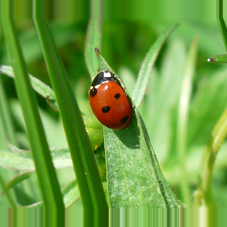
\includegraphics[width=2cm]{data/ladybug.png}
            };
            \draw[-Latex] (input) -- (model);
        }
        \only<1-2>{
            \node[anchor=west] (output) at ($ (model.east) + (0.77, 0) $) {
                ladybug
            };
            \draw[-Latex] (model) -- (output);
        }
        \only<2>{
            \node[anchor=north, text=red] (pass) at (model.south) {
                \textbf{\textit{Backward pass}}
            };
            \draw[stealth-, red] (pass.south west) -- (pass.south east);

            \node[] at (0, -2.5) {
                $R^{i-1}_j=\sum\limits_{k} \dfrac{n^{(i-1)}_jw^{(i-1)}_{jk}}{\sum\limits_{l} n^{(i-1)}_lw^{(i-1)}_{lk}}R^i_k$
            };
        }
        \only<3->{
            \node[anchor=west, text=red] (output) at ($ (model.east) + (0.77, 0) $) {
                ladybug
            };
            \draw[Latex-,red] (model) -- (output);}
    \end{tikzpicture}

\end{frame}

    

\definecolor{cases-default}{HTML}{EB5353}
\definecolor{controls-default}{HTML}{0079FF}
\definecolor{healthy-default}{HTML}{36AE7C}

\newcommand{\scannersubplot}[3]{
    \nextgroupplot[
            axis lines=center,
            axis y line=none,
            xmin=46,
            xmax=99,
            ymin=-1.65,
            ymax=1.5,
            xmajorticks=false,
            axis line style={-}
        ]

            \addplot[name path=zero, draw=none] coordinates {(46, 0) (99, 0)};
            \addplot[
                name path=fcases,
                draw=cases-default,
                very thick
            ] table [
                col sep=comma,
                x=x,
                y=F-cases
            ]{#1};
            \addplot[fill=cases-default, opacity=0.2] fill between [of=zero and fcases];

            \addplot[
                name path=fcontrols,
                draw=controls-default,
                very thick
            ] table [
                col sep=comma,
                x=x,
                y=F-controls
            ]{#1};
            \addplot[fill=controls-default, opacity=0.2] fill between [of=zero and fcontrols];

            \addplot[
                name path=mcases,
                draw=cases-default,
                very thick
            ] table [
                col sep=comma,
                x=x,
                y expr=\thisrow{M-cases} * -1
            ]{#1};
            \addplot[fill=cases-default, opacity=0.2] fill between [of=zero and mcases];

            \addplot[
                name path=mcontrols,
                draw=controls-default,
                very thick
            ] table [
                col sep=comma,
                x=x,
                y expr=\thisrow{M-controls} * -1
            ]{#1};
            \addplot[fill=controls-default, opacity=0.2] fill between [of=zero and mcontrols];

            \node[anchor=south] at (axis cs: 72.5,0.85) {\tiny{#2}};
            \node[anchor=north] at (axis cs: 72.5,-1) {\tiny{\textbf{n=#3}}};
}

\newsavebox{\fulldementiadataset}
\sbox{\fulldementiadataset}{
    \begin{tikzpicture}
        \begin{axis}[
            width=\textwidth,
            height=0.35\textwidth,
            xmin=46,
            xmax=99,
            ymin=-1.6,
            ymax=1.2,
            xtick={55,60,65,70,75,80,85,90,95},
            axis lines=center,
            axis y line=none,
            clip=false
        ]
            \addplot[name path=zero, draw=none] coordinates {(47,0) (97,0)};

            \addplot[
                name path=fcases,
                draw=cases-default,
                very thick
            ] table [
                col sep=comma,
                x=x,
                y=F-cases
            ]{data/dementia_dataset/dementia_full.csv};\label{trace:cases}
            \addplot[fill=cases-default, opacity=0.2] fill between [of=zero and fcases];

            \addplot[
                name path=fcontrols,
                draw=controls-default,
                very thick
            ] table [
                col sep=comma,
                x=x,
                y=F-controls
            ]{data/dementia_dataset/dementia_full.csv};\label{trace:controls}
            \addplot[fill=controls-default, opacity=0.2] fill between [of=zero and fcontrols];

            \addplot[
                name path=mcases,
                draw=cases-default,
                very thick
            ] table [
                col sep=comma,
                x=x,y
                expr=\thisrow{M-cases} * -1
            ]{data/dementia_dataset/dementia_full.csv};
            \addplot[fill=cases-default, opacity=0.2] fill between [of=zero and mcases];

            \addplot[
                name path=mcontrols,
                draw=controls-default,
                very thick
            ] table [
                col sep=comma,
                x=x,
                y expr=\thisrow{M-controls} * -1
            ]{data/dementia_dataset/dementia_full.csv};
            \addplot[fill=controls-default, opacity=0.2] fill between [of=zero and mcontrols];

            \node[anchor=south west] at (axis cs: 46, 0.07) {\textbf{FEMALE}};
            \node[anchor=north west] at (axis cs: 46, -0.07) {\textbf{MALE}};
            \node[anchor=south, font=\footnotesize\selectfont, align=center] (n) at (axis cs: 72.5,-1.8) {n=1708};
            \node[anchor=south west,font=\footnotesize\selectfont, align=left] at ($(n.south east) + (110,0) $) {
                \ref{trace:controls} Controls\\[-0.1cm]
                \ref{trace:cases} Patients
            };
        \end{axis}
    \end{tikzpicture}
}

\newsavebox{\dementiasubsets}
\sbox{\dementiasubsets}{
    \begin{tikzpicture}
        \begin{groupplot}[
            group style={
                group size=5 by 2,
                horizontal sep=0.25cm,
                vertical sep=0.25cm
            },
            height=0.28\textwidth,
            width=0.314\textwidth
        ]
            \scannersubplot{data/dementia_dataset/dementia_ADNI_30T.csv}{ADNI 3.0T}{506}
            \scannersubplot{data/dementia_dataset/dementia_oasis3_30T.csv}{OASIS3 3.0T}{438}
            \scannersubplot{data/dementia_dataset/dementia_ADNI_15T.csv}{ADNI 1.5T}{290}
            \scannersubplot{data/dementia_dataset/dementia_Oslo_GE750.csv}{Oslo GE750}{226}
            \scannersubplot{data/dementia_dataset/dementia_AIBL_10.csv}{AIBL Site 1}{92}
            \scannersubplot{data/dementia_dataset/dementia_addneuromed_GE_MEDICAL_SYSTEMS.csv}{ANM GE}{74}
            \scannersubplot{data/dementia_dataset/dementia_miriad_15_T_Signa.csv}{MIRIAD}{38}
            \scannersubplot{data/dementia_dataset/dementia_AIBL_20.csv}{AIBL Site 2}{22}
            \scannersubplot{data/dementia_dataset/dementia_addneuromed_PICKER_International_Inc.csv}{ANM Picker}{12}
            \scannersubplot{data/dementia_dataset/dementia_oasis3_15T.csv}{OASIS3 1.5T}{10}
        \end{groupplot}
    \end{tikzpicture}
}

\newcommand{\dementiapredictions}{
    \begin{tikzpicture}
        \begin{axis}[
            height=3.5cm,
            width=8cm,
            xlabel=\textbf{Prediction},
            ylabel=\textbf{Cohort},
            xtick={0, 1},
            xticklabels={Healthy, Dementia},
            ytick={1, 2},
            yticklabels={Controls, Patients},
            xtick pos=bottom,
            ytick pos=left,
            xlabel style={
                at={(axis description cs:0.5,-0.1)}
            }
        ]
            \addplot+[
                boxplot prepared={
                    median=0.08,
                    upper quartile=0.21,
                    lower quartile=0.04,
                    upper whisker=0.48,
                    lower whisker=0
                },
                draw=black,
                fill=controls-default
            ] coordinates {};
            \addplot+[
                only marks,
                mark=*,
                draw=black,
                fill=red,
                mark options={
                    fill=controls-default,
                    opacity=0.1
                }
            ] coordinates {
                (0.50446737, 1)
                (0.50301045, 1)
                (0.8623527, 1)
                (0.5224974, 1)
                (0.7995614, 1)
                (0.72703606, 1)
                (0.6828119, 1)
                (0.9235332, 1)
                (0.49864507, 1)
                (0.76377636, 1)
                (0.8327935, 1)
                (0.9408187, 1)
                (0.98629504, 1)
                (0.66696477, 1)
                (0.80282503, 1)
                (0.86055464, 1)
                (0.90125066, 1)
                (0.98291415, 1)
                (0.6314192, 1)
                (0.77041364, 1)
                (0.5979652, 1)
                (0.7827456, 1)
                (0.9518579, 1)
                (0.99622357, 1)
                (0.99328387, 1)
                (0.69867474, 1)
                (0.6601426, 1)
                (0.75362796, 1)
                (0.7569201, 1)
                (0.5105941, 1)
                (0.6899047, 1)
                (0.71893066, 1)
                (0.57259643, 1)
                (0.9819919, 1)
                (0.5338644, 1)
                (0.57063895, 1)
                (0.6915874, 1)
                (0.53687215, 1)
                (0.6003495, 1)
                (0.54097295, 1)
                (0.9115054, 1)
                (0.6653496, 1)
                (0.8144589, 1)
                (0.9939644, 1)
                (0.960153, 1)
                (0.9648322, 1)
                (0.6721609, 1)
                (0.48370066, 1)
                (0.8403382, 1)
                (0.71983075, 1)
                (0.72373754, 1)
                (0.97700036, 1)
                (0.78138167, 1)
                (0.5741908, 1)
                (0.55037045, 1)
                (0.60542965, 1)
                (0.74589527, 1)
                (0.66231793, 1)
                (0.9737994, 1)
                (0.97011316, 1)
                (0.73134863, 1)
                (0.73491704, 1)
                (0.9212756, 1)
                (0.73766065, 1)
                (0.7221923, 1)
                (0.9278477, 1)
                (0.998459, 1)
                (0.5751162, 1)
                (0.64807665, 1)
                (0.9903199, 1)
                (0.6751649, 1)
                (0.6104782, 1)
                (0.99662316, 1)
                (0.6976316, 1)
                (0.55103743, 1)
                (0.99890363, 1)
                (0.9999541, 1)
                (0.75735366, 1)
                (0.6077365, 1)
                (0.970043, 1)
                (0.85138136, 1)
                (0.5465968, 1)
                (0.99242157, 1)
                (0.9150392, 1)
                (0.8648588, 1)
                (0.52396196, 1)
                (0.75622225, 1)
                (0.7811335, 1)
                (0.9982332, 1)
                (0.59327227, 1)
                (0.9919817, 1)
                (0.8797925, 1)
                (0.8329868, 1)
                (0.5257523, 1)
                (0.82573485, 1)
                (0.5419094, 1)
                (0.7384044, 1)
                (0.96513677, 1)
                (0.5511491, 1)
                (0.93219143, 1)
                (0.81861705, 1)
                (0.54127866, 1)
            };
            \addplot+[
                boxplot prepared={
                    median=0.95,
                    upper quartile=0.99,
                    lower quartile=0.67,
                    upper whisker=1,
                    lower whisker=0.20
                },
                draw=black,
                fill=cases-default
            ] coordinates {};
            \addplot+[
                only marks,
                mark=*,
                draw=black,
                mark options={
                    fill=cases-default,
                    opacity=0.1
                }
            ] coordinates {
                (0.11294349, 2)
                (0.14141159, 2)
                (0.047518212, 2)
                (0.035283785, 2)
                (0.18220703, 2)
                (0.08105849, 2)
                (0.18563321, 2)
                (0.18436697, 2)
                (0.18438818, 2)
                (0.106455594, 2)
                (0.16512504, 2)
                (0.037674535, 2)
                (0.116673164, 2)
                (0.022512339, 2)
                (0.04461377, 2)
                (0.01521102, 2)
                (0.081032276, 2)
                (0.03708474, 2)
                (0.041679956, 2)
                (0.04825165, 2)
                (0.07813377, 2)
                (0.19328135, 2)
                (0.059010953, 2)
                (0.087162666, 2)
                (0.17256281, 2)
                (0.115628816, 2)
                (0.049699314, 2)
                (0.022067336, 2)
                (0.09318608, 2)
                (0.043719042, 2)
                (0.09821392, 2)
                (0.049812526, 2)
                (0.053025473, 2)
                (0.026935639, 2)
                (0.07707973, 2)
                (0.089302234, 2)
                (0.11172331, 2)
                (0.14193982, 2)
                (0.04984702, 2)
                (0.11108907, 2)
                (0.04263115, 2)
                (0.079762705, 2)
                (0.03469864, 2)
                (0.017143656, 2)
                (0.048551403, 2)
                (0.122921765, 2)
                (0.11892662, 2)
                (0.09896589, 2)
                (0.1929691, 2)
                (0.037067875, 2)
                (0.19084817, 2)
                (0.11711612, 2)
                (0.13370761, 2)
                (0.11053958, 2)
                (0.048200555, 2)
                (0.012198591, 2)
                (0.0012190987, 2)
                (0.0006263061, 2)
                (0.021543678, 2)
                (0.15559466, 2)
                (0.019410677, 2)
                (0.12729207, 2)
                (0.011612348, 2)
                (0.081171475, 2)
                (0.030508395, 2)
                (0.040783383, 2)
                (0.00087664387, 2)
                (0.17205802, 2)
                (0.06274164, 2)
                (0.09376377, 2)
                (0.15760471, 2)
                (0.1451328, 2)
                (0.14305037, 2)
                (0.13085763, 2)
                (0.0953999, 2)
                (0.091083504, 2)
                (0.19047028, 2)
                (0.18113527, 2)
                (0.10130572, 2)
                (0.15542361, 2)
                (0.09163013, 2)
                (0.13151047, 2)
                (0.071478605, 2)
                (0.071758784, 2)
                (0.1452744, 2)
                (0.09954041, 2)
                (0.07047755, 2)
                (0.15672913, 2)
            };
        \end{axis}
    \end{tikzpicture}
}

\newsavebox{\predictionbox}
\sbox{\predictionbox}{
    \dementiapredictions
}

\begin{frame}[t]{XAI and dementia}
    \centering
    \vfill

    \begin{tikzpicture}
        \node[] at (-5.25, 3.25) {};
        \node[] at (5.25, -3.25) {};

        \only<1>{
            \node[anchor=north] at (0, 3.35) {
                \usebox{\fulldementiadataset}
            };
            \node[] at (0, -1.1) {
                \usebox{\dementiasubsets}
            };

            \node[anchor=south, font=\tiny, text width=10.5cm, align=flush center] at (0, -3.75) {
            Leonardsen et al., \textit{Constructing personalized characterizations of structural brain aberrations in patients with dementia using explainable artificial intelligence} (2024), \url{https://www.nature.com/articles/s41746-024-01123-7}
            };
        }
        \only<2-6>{
            \inputside{-4}{1.5}{1.5cm}
        }
        \only<3->{
            \node[
                font=\linespread{0.9}\selectfont,
                align=left,
                anchor=west
            ] (output) at (3.4, 1.5) {
                Dementia\\patient\\or healthy \\control?
            };
        }
        \only<4-6>{
            \cnnarrow{(input.east)}{($ (input.center) + (2, 0) $)}{black}
            \cnn{-2.3}{1.5}{0.066}{0.15}{black}{1}
            \cnnarrow{($ (output.west) - (0.54, 0) $)}{($ (output.west) + (0.1, 0) $)}{black}
        }
        \only<5>{
            \node[] at (-0.6, -2) {
                \usebox{\predictionbox}
            };
        }
        \only<7>{
            \heatmapside{-4}{1.5}{1.5cm}
            \lrparrow{($ (input.center) + (2, 0) $)}{(input.east)}{black}
            \lrp{-2.3}{1.5}{0.066}{0.15}
            \lrparrow{($ (output.west) + (0.1, 0) $)}{($ (output.west) - (0.54, 0) $)}{black}

        }
    \end{tikzpicture}
\end{frame}

\newcommand{\annotation}[4]{
    \node[anchor=#4,align=center,font=\scriptsize\linespread{0.8}\selectfont,inner sep=2.5pt] at (axis cs: #2,#3) {#1};
}

\newsavebox{\regions}
\sbox{\regions}{
    \begin{tikzpicture}
        \begin{axis}[
            width=\textwidth,
            height=0.6\textwidth,
            ylabel=Human-rated importance,
            xlabel=AI-rated importance,
            ticks=none,
            xmin=0,
            xmax=1.25,
            ymin=0,
            ymax=1.1,
            axis y line=left,
            axis x line=bottom,
            ylabel style={
                align=center
            }
        ]
            \addplot[only marks, fill=babalightblue, draw=black] table [col sep=comma, x=lrp, y=ale] {data/test_mean.csv};
            \annotation{Left Accumbens}{0.906}{1}{south}
            \annotation{Right Accumbens}{0.731}{0.914}{north}
            \annotation{Left Amygdala}{1}{0.719}{south}
            \annotation{Right Amygdala}{0.767}{0.699}{north}
            \annotation{Parahippocampal\\Gyrus}{0.594}{0.415}{south}
            \annotation{Heschl's\\Gyrus}{0.785}{0.276}{south}
            \annotation{Lingual\\Gyrus}{0.517}{0.312}{north}
            \annotation{Planum\\Temporale}{0.407}{0.159}{north}
        \end{axis}
    \end{tikzpicture}
}

\begin{frame}{XAI and dementia: Validation}
    \begin{tikzpicture}
        \node[] at (-5.25, 3.5) {};
        \node[] at (5.25, -3.5) {};

        \only<1>{
            \node[
				minimum height=0.41\textwidth,
				minimum width=0.32\textwidth,
				fill=black,
                anchor=west
			] (box1) at (-5.25, 0) {};
			\node[anchor=south] at (box1.south) {
				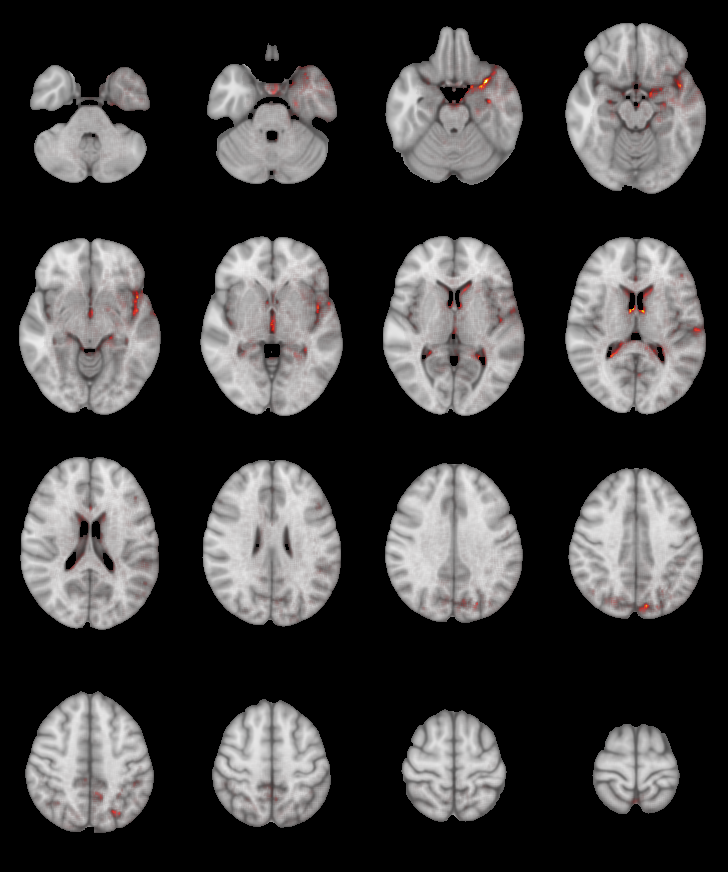
\includegraphics[width=0.31\textwidth]{data/subject1.png}
			};
			\node[anchor=north,inner sep=2pt, text=white, font=\footnotesize] at (box1.north) {Patient 1};

			\node
				[minimum height=0.41\textwidth,
				minimum width=0.32\textwidth,
				fill=black,
				anchor=west
			] (box2) at ($ (box1.east) + (0.05,0) $) {};
			\node[anchor=south] at (box2.south) {
				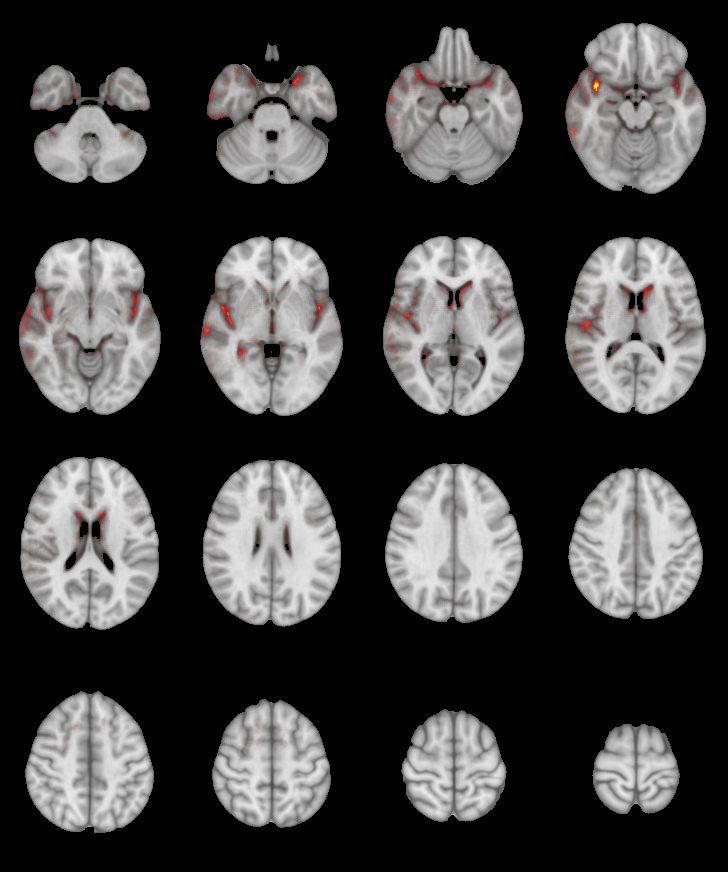
\includegraphics[width=0.31\textwidth]{data/subject2.png}
			};
			\node[anchor=north,inner sep=3pt, text=white, font=\footnotesize] at (box2.north) {Patient 2};

			\node
				[minimum height=0.41\textwidth,
				minimum width=0.32\textwidth,
				fill=black,
				anchor=west
			] (box3) at ($ (box2.east) + (0.05,0) $) {};
			\node[anchor=south] at (box3.south) {
				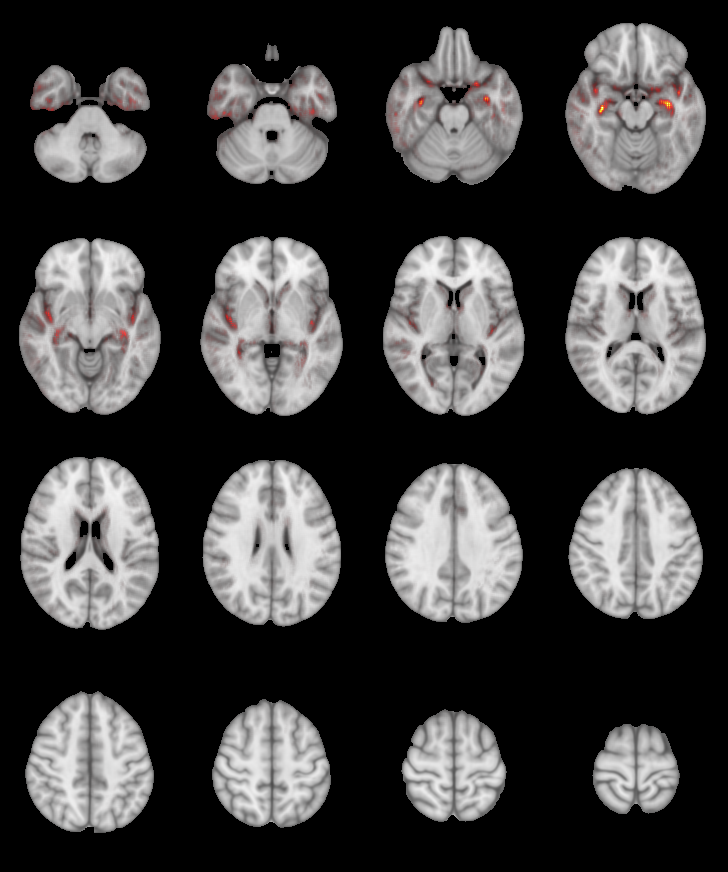
\includegraphics[width=0.31\textwidth]{data/subject3.png}
			};
			\node[anchor=north,inner sep=3pt, text=white, font=\footnotesize] at (box3.north) {Patient 3};
        }

        \only<2-3>{
            \node[label={[text depth=0]above:Explainable AI}] at (-2.25, 0) {
				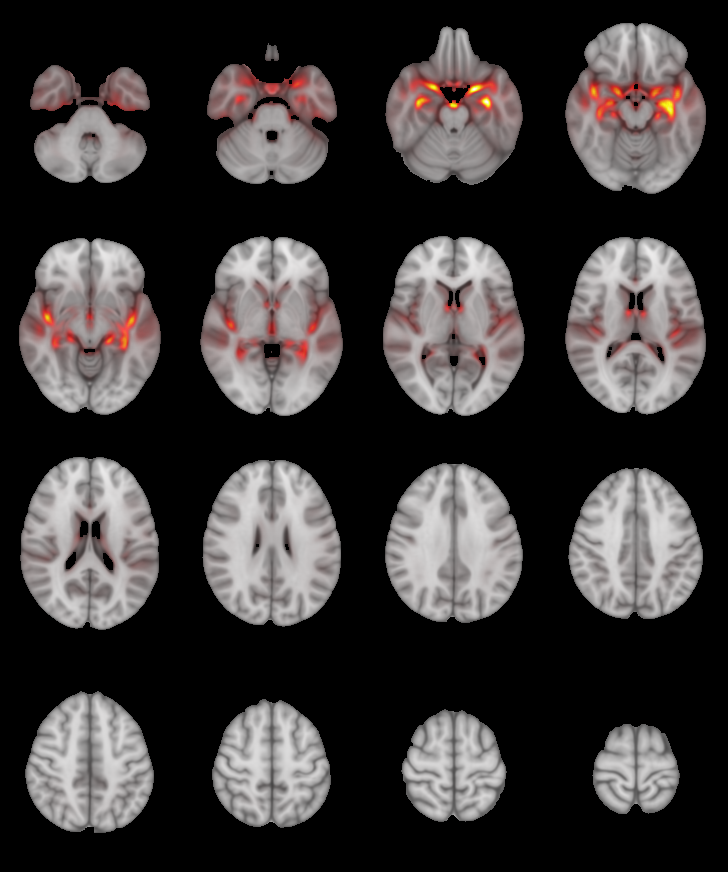
\includegraphics[width=0.31\textwidth]{data/dementia.png}
			};
        }
        \only<3>{
			\node[label={[text depth=0]above:Human researchers}] at (2.25, 0) {
				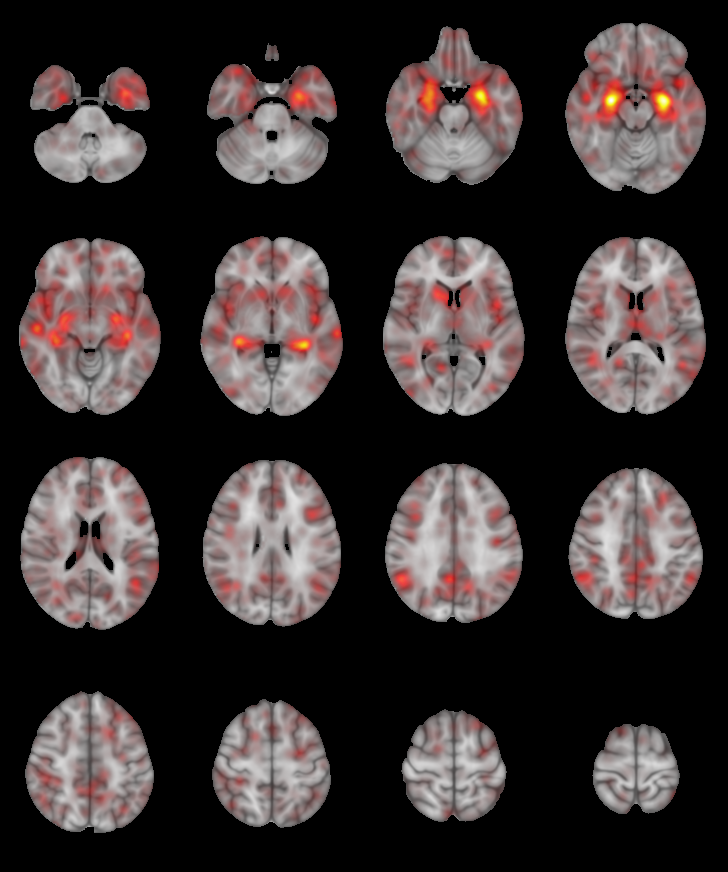
\includegraphics[width=0.31\textwidth]{data/ALE.png}
			};
        }
        \only<4>{
            \node[] at (0, 0) {
                \usebox{\regions}
            };
        }

    \end{tikzpicture}
\end{frame}

\definecolor{baseline}{HTML}{FAEAB1}
\definecolor{preds}{HTML}{E5BA73}
\definecolor{maps}{HTML}{C58940}

\newcommand{\prognostic}{
    \begin{tikzpicture}
        \begin{axis}[
            height=2.9cm,
            width=4.08cm,
            xmajorticks=false,
            xmin=0.5,
            xmax=5.5,
            ymin=0,
            ymax=1,
            ylabel=\footnotesize{AUC},
            ymajorticks=false,
            ymajorgrids=true
        ]

            \addplot[mark=*, draw=black, mark options={fill=maps}] coordinates {
                (1, 0.743)
                (2, 0.786)
                (3, 0.808)
                (4, 0.867)
                (5, 0.903)
            };

        \end{axis}
    \end{tikzpicture}
}


\newsavebox{\prognosticheatmaps}
\sbox{\prognosticheatmaps}{
    \prognostic
}

\newcommand{\mciconcept}[1]{
    \begin{tikzpicture}
        \begin{axis}[
            height=0.6\textwidth,
            width=0.8\textwidth,
            xlabel={Age},
            ylabel={Cognitive function},
            ticks=none,
            axis x line=bottom,
            axis y line=left,
            y axis line style={-|},
            xmin=0,
            xmax=1.4,
            ymin=0,
            ymax=1,
            clip=false
        ]
            \addplot[draw=healthy-default, smooth, line width=4pt, opacity=0.5] coordinates {
                (0, 0.9)
                (0.25, 0.87)
                (0.5, 0.77)
                (0.6, 0.72)
                (0.8, 0.63)
                (0.9, 0.72)
                (1.4, 0.67)
            };
            \addplot[draw=controls-default, smooth, line width=4pt, opacity=0.5] coordinates {
                (0, 0.9)
                (0.25, 0.87)
                (0.5, 0.77)
                (0.6, 0.72)
                (0.8, 0.63)
                (0.9, 0.61)
                (1.4, 0.54)
            };
            \addplot[draw=cases-default, smooth, line width=4pt, opacity=0.5] coordinates {
                (0, 0.9)
                (0.25, 0.87)
                (0.5, 0.77)
                (0.6, 0.72)
                (0.8, 0.625)
                (1.1, 0.48)
                (1.4, 0.3)
            };
            \addplot[dashed] coordinates {
                (0, 0.65)
                (1.4, 0.65)
            };
            \addplot[dashed] coordinates {
                (0, 0.4)
                (1.4, 0.4)
            };
            \node[anchor=south west] at (axis cs: 0, 0.64) {\footnotesize{Normal cognition}};
            \node[anchor=north west] at (axis cs: 0, 0.66) {\footnotesize{Mild cognitive impairment}};
            \node[anchor=north west] at (axis cs: 0, 0.41) {\footnotesize{Dementia}};

            \ifnum#1<3
                \node[anchor=west] at (axis cs: 1.4, 0.67) {\textcolor{healthy-default}{\footnotesize{Improving (n=80)}}};
                \node[anchor=west] at (axis cs: 1.4, 0.53) {\textcolor{controls-default}{\footnotesize{Stable (n=754)}}};
                \node[anchor=west] at (axis cs: 1.4, 0.3) {\textcolor{cases-default}{\footnotesize{Progressive (n=354)}}};
            \fi

            \ifnum#1>0
                \draw[-stealth, red, thick] (axis cs: 0.8, 0.8) -- (axis cs: 0.8, 0.67);
                \node[anchor=south] at (axis cs: 0.8, 0.8) {\textcolor{red}{\footnotesize{t}}};
            \fi

            \ifnum#1>1
                \draw[densely dotted] (axis cs: 0.9, 0.8) -- (axis cs: 0.9, 0.3);
                \draw[densely dotted] (axis cs: 1, 0.8) -- (axis cs: 1, 0.3);
                \draw[densely dotted] (axis cs: 1.1, 0.8) -- (axis cs: 1.1, 0.3);
                \draw[densely dotted] (axis cs: 1.2, 0.8) -- (axis cs: 1.2, 0.3);
                \draw[densely dotted] (axis cs: 1.3, 0.8) -- (axis cs: 1.3, 0.3);
                \node[anchor=south] at (axis cs: 0.9, 0.8) {\footnotesize{t+1}};
                \node[anchor=south] at (axis cs: 1, 0.8) {\footnotesize{t+2}};
                \node[anchor=south] at (axis cs: 1.1, 0.8) {\footnotesize{t+3}};
                \node[anchor=south] at (axis cs: 1.2, 0.8) {\footnotesize{t+4}};
                \node[anchor=south] at (axis cs: 1.3, 0.8) {\footnotesize{t+5}};
            \fi

            \ifnum#1=3
                \node[] at (axis cs: 1.025, 0.155) {
                    \usebox{\prognosticheatmaps}
                };
			    \node[anchor=west] at (axis cs: 1.34, 0.262) {\footnotesize{0.90}};
            \fi

        \end{axis}
    \end{tikzpicture}
}

\newsavebox{\mcitrajectories}
\sbox{\mcitrajectories}{
    \mciconcept{0}
}
\newsavebox{\mcitimepoint}
\sbox{\mcitimepoint}{
    \mciconcept{1}
}
\newsavebox{\mcifuture}
\sbox{\mcifuture}{
    \mciconcept{2}
}
\newsavebox{\mciheatmaps}
\sbox{\mciheatmaps}{
    \mciconcept{3}
}

\newcommand{\mriwidth}{2.2cm}
\newcommand{\gap}{0.00cm}

\definecolor{color0}{rgb}{0.62, 0.004, 0.259}
\definecolor{color1}{rgb}{0.755, 0.154, 0.291}
\definecolor{color2}{rgb}{0.866, 0.29, 0.298}
\definecolor{color3}{rgb}{0.943, 0.406, 0.268}
\definecolor{color4}{rgb}{0.975, 0.557, 0.323}
\definecolor{color5}{rgb}{0.993, 0.709, 0.403}
\definecolor{color6}{rgb}{0.995, 0.832, 0.506}
\definecolor{color7}{rgb}{0.998, 0.926, 0.625}
\definecolor{color8}{rgb}{0.998, 0.999, 0.746}
\definecolor{color9}{rgb}{0.937, 0.975, 0.65}
\definecolor{color10}{rgb}{0.838, 0.935, 0.609}
\definecolor{color11}{rgb}{0.693, 0.876, 0.639}
\definecolor{color12}{rgb}{0.527, 0.811, 0.645}
\definecolor{color13}{rgb}{0.368, 0.725, 0.662}
\definecolor{color14}{rgb}{0.24, 0.582, 0.721}
\definecolor{color15}{rgb}{0.267, 0.441, 0.698}
\definecolor{color16}{rgb}{0.369, 0.31, 0.635}

\newcommand{\correlationplot}[4]{
    \begin{tikzpicture}
        \begin{axis}[
            height=1.71 * \mriwidth,
            width=1.71 * \mriwidth,
            xmajorticks=false,
            ylabel=#3,
            ytick={0, 2, 4, 6, 8},
            yticklabels=#2,
            xmin=-1,
            xmax=17,
            ymin=0,
            ymax=9,
            every tick label/.append style={font=\tiny},
            ytick pos=left,
            scatter/classes={
                ADNI_EF={color0, draw=black},
                ADNI_MEM={color1, draw=black},
                CDCARE={color2, draw=black},
                CDCOMMUN={color3, draw=black},
                CDGLOBAL={color4, draw=black},
                CDHOME={color5, draw=black},
                CDJUDGE={color6, draw=black},
                CDMEMORY={color7, draw=black},
                CDORIENT={color8, draw=black},
                FAQTOTAL={color9, draw=black},
                GDTOTAL={color10, draw=black},
                MMSCORE={color11, draw=black},
                NPISCORE={color12, draw=black},
                PHC_EXF={color13, draw=black},
                PHC_LAN={color14, draw=black},
                PHC_MEM={color15, draw=black},
                PHC_VSP={color16, draw=black}
            },
            y label style={at={(-0.1,0.5)}},
            ymajorgrids=true,
            ytick style={draw=none},
            clip=false,
            grid style={draw=gray!20},
            axis line style={draw=gray!70}
        ]
            \addplot[
                only marks,
                scatter,
                scatter src=explicit symbolic
            ] table [
                col sep=comma,
                x=index,
                y=component_#1,
                meta=symptom
            ] {data/correlations.csv};
            \addplot[dashed,red, thick] coordinates {
                (-1, 2.76)
                (17, 2.76)
            };
            #4
        \end{axis}
    \end{tikzpicture}
}

\newsavebox{\firstcorrelations}
\sbox{\firstcorrelations}{%
    \correlationplot{0}{{0, 2, 4, 6, 8}}{\scriptsize{$-log_{10}(p)$}}{
        \node[] at (axis cs: 14, 6.19) {\tiny{PHC\_LAN}};
    }
}
\newsavebox{\secondcorrelations}
\sbox{\secondcorrelations}{%
    \correlationplot{1}{{,,}}{{}}{
        \node[] at (axis cs: 9, 3.74) {\tiny{FAQTOTAL}};
    }
}
\newsavebox{\thirdcorrelations}
\sbox{\thirdcorrelations}{%
    \correlationplot{2}{{,,}}{{}}{
        \node[] at (axis cs: 0, 6.44) {\tiny{ADNI\_EF}};
        \node[] at (axis cs: 13, 7.95) {\tiny{PHC\_EXF}};
    }
}
\newsavebox{\fourthcorrelations}
\sbox{\fourthcorrelations}{%
    \correlationplot{3}{{,,}}{{}}{
        \node[] at (axis cs: 0, 9.02) {\tiny{ADNI\_EF}};
        \node[] at (axis cs: 13, 8.75) {\tiny{PHC\_EXF}};
        \node[] at (axis cs: 14, 5.84) {\tiny{PHC\_LAN}};
        \node[] at (axis cs: 6, 5.18) {\tiny{CDJUDGE}};
        \node[] at (axis cs: 11, 3.99) {\tiny{MMSCORE}};
    }
}

\newcommand{\cognitiveplot}[1]{
    \hspace{-0.6cm}
    \begin{tikzpicture}
        \node[] (first) at (0, 0) {
            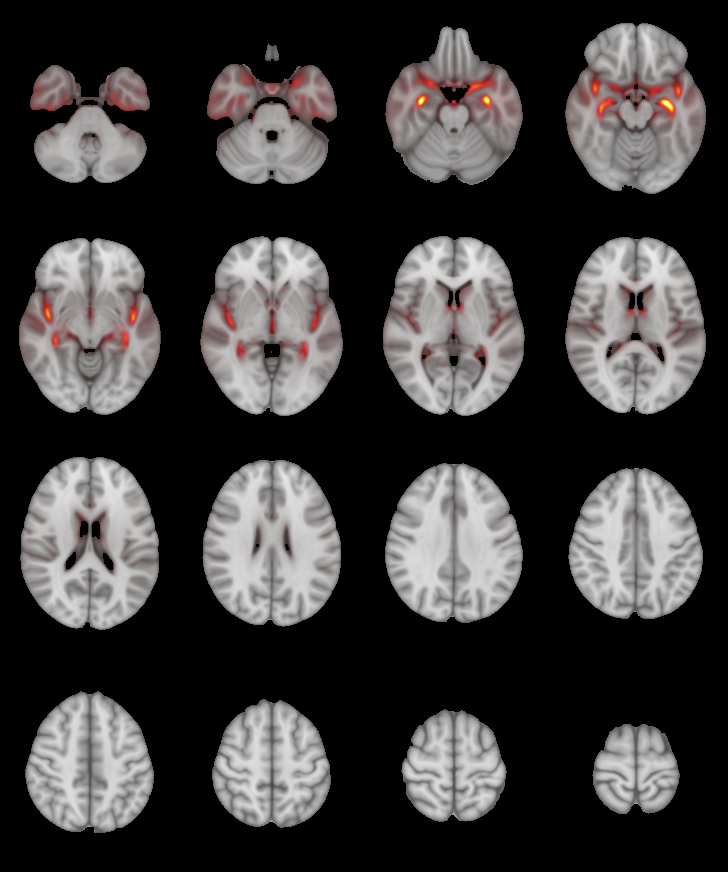
\includegraphics[
                width=\mriwidth,
                clip=true,
                trim = 192mm 232mm 0mm 0mm
            ]{data/components/component_0.png}
        };

        \node[anchor=west] (second) at ($ (first.east) + (\gap, 0) $) {
            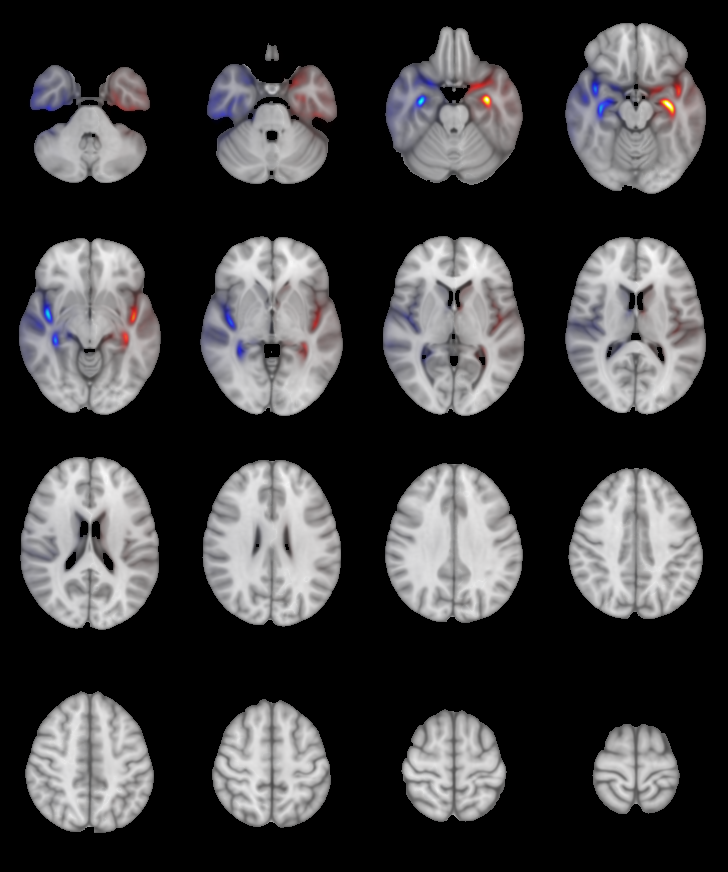
\includegraphics[
                width=\mriwidth,
                clip=true,
                trim = 192mm 232mm 0mm 0mm
            ]{data/components/component_1.png}
        };

        \node[anchor=west] (third) at ($ (second.east) + (\gap, 0) $) {
            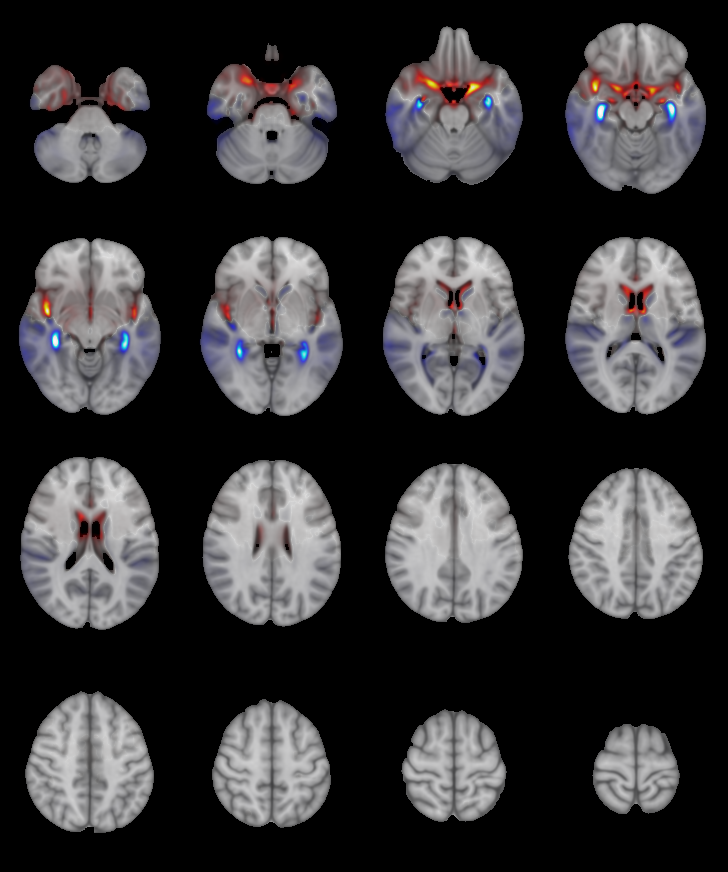
\includegraphics[
                width=\mriwidth,
                clip=true,
                trim = 192mm 232mm 0mm 0mm
            ]{data/components/component_2.png}
        };

        \node[anchor=west] (fourth) at ($ (third.east) + (\gap, 0) $) {
            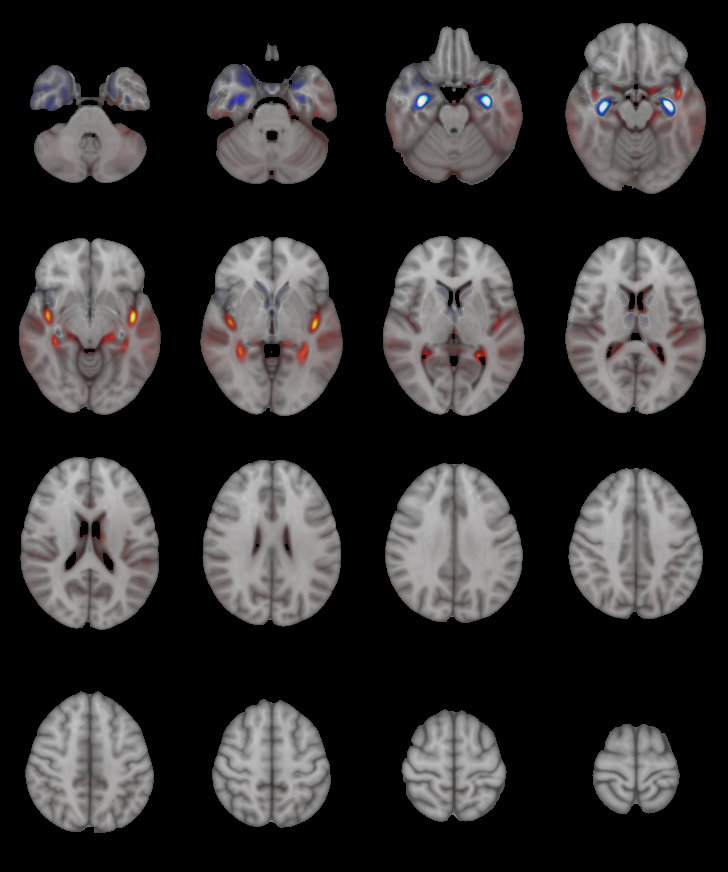
\includegraphics[
                width=\mriwidth,
                clip=true,
                trim = 192mm 232mm 0mm 0mm
            ]{data/components/component_3.png}
        };

        \ifnum#1=1
            \node[anchor=north west] (first-correlation) at ($ (first.south west) + (-0.86, 0.1) $) {
                \usebox{\firstcorrelations}
            };
            \node[anchor=north west] (second-correlation) at ($ (first-correlation.north east) - (0.76, 0) $) {
                \usebox{\secondcorrelations}
            };
            \node[anchor=north west] (third-correlation) at ($ (second-correlation.north east) - (0.71, 0) $) {
                \usebox{\thirdcorrelations}
            };
            \node[anchor=north west] (fourth-correlation) at ($ (third-correlation.north east) - (0.74, -0.21) $) {
                \usebox{\fourthcorrelations}
            };
        \fi

    \end{tikzpicture}
    \hspace{-0.6cm}
}

\newsavebox{\cognitiveheatmaps}
\sbox{\cognitiveheatmaps}{
    \cognitiveplot{0}
}

\newsavebox{\cognitivecorrelations}
\sbox{\cognitivecorrelations}{
    \cognitiveplot{1}
}

\begin{frame}{XAI and dementia: Clinical applications}
    \begin{tikzpicture}
        \node[] at (-5.25, 3.5) {};
        \node[] at (5.5, -3.5) {};

        \only<1>{
                        \node[
				minimum height=0.41\textwidth,
				minimum width=0.32\textwidth,
				fill=black,
                anchor=west
			] (box1) at (-5.25, 0) {};
			\node[anchor=south] at (box1.south) {
				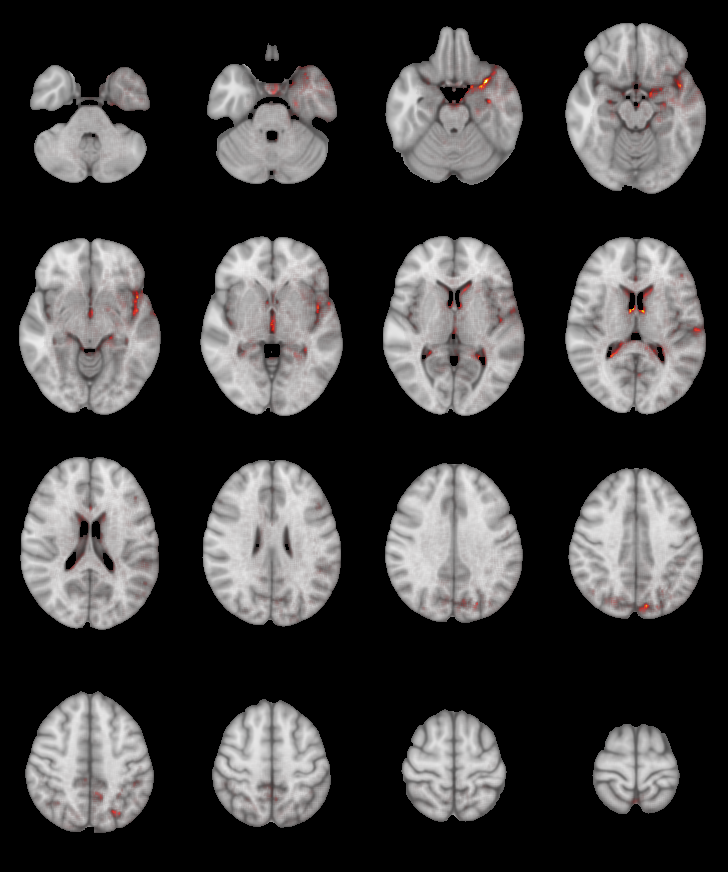
\includegraphics[width=0.31\textwidth]{data/subject1.png}
			};
			\node[anchor=north,inner sep=2pt, text=white, font=\footnotesize] at (box1.north) {Patient 1};

			\node
				[minimum height=0.41\textwidth,
				minimum width=0.32\textwidth,
				fill=black,
				anchor=west
			] (box2) at ($ (box1.east) + (0.05,0) $) {};
			\node[anchor=south] at (box2.south) {
				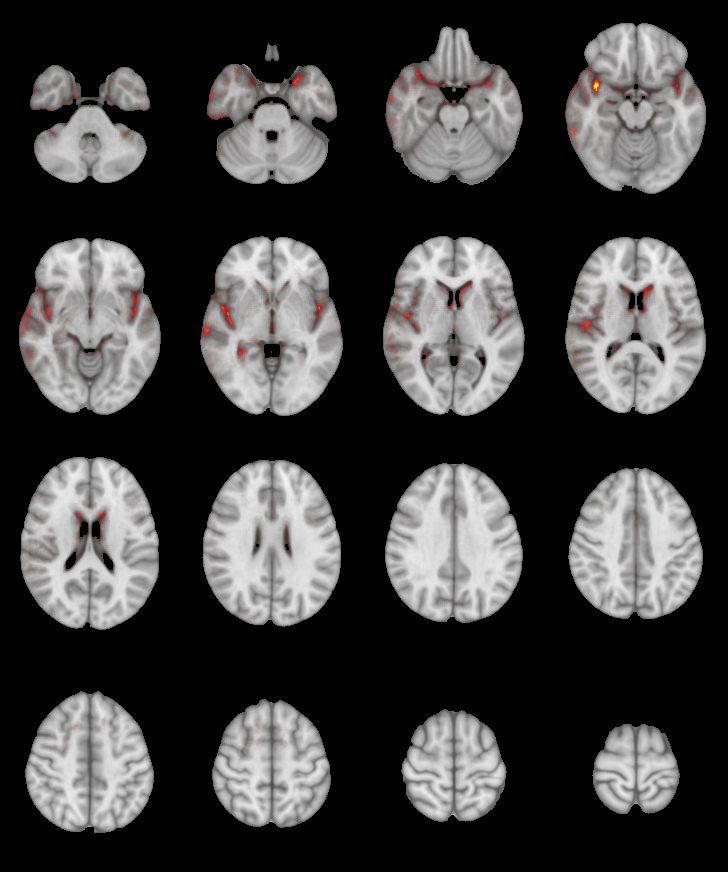
\includegraphics[width=0.31\textwidth]{data/subject2.png}
			};
			\node[anchor=north,inner sep=3pt, text=white, font=\footnotesize] at (box2.north) {Patient 2};

			\node
				[minimum height=0.41\textwidth,
				minimum width=0.32\textwidth,
				fill=black,
				anchor=west
			] (box3) at ($ (box2.east) + (0.05,0) $) {};
			\node[anchor=south] at (box3.south) {
				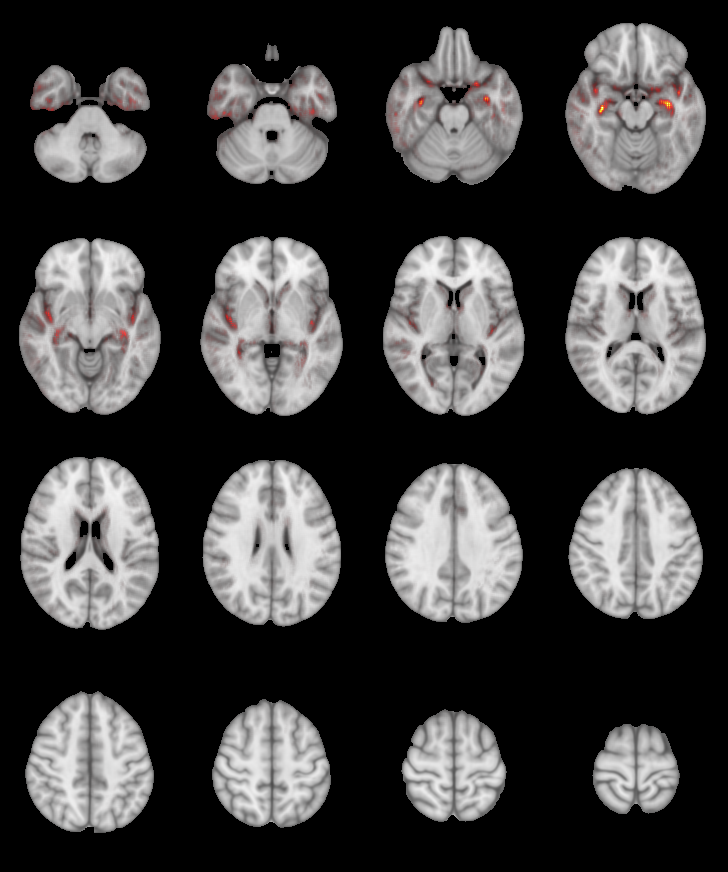
\includegraphics[width=0.31\textwidth]{data/subject3.png}
			};
			\node[anchor=north,inner sep=3pt, text=white, font=\footnotesize] at (box3.north) {Patient 3};
        }

        \only<2>{
            \node[] at (0, 0) {
                \usebox{\mcitrajectories}
            };
        }

        \only<3>{
            \node[anchor=west] at (-5, 0) {
                \usebox{\mcitimepoint}
            };
        }
        \only<4>{
            \node[anchor=west] at (-5, 0) {
                \usebox{\mcifuture}
            };
        }
        \only<5>{
            \node[anchor=west] at (-5, 0) {
                \usebox{\mciheatmaps}
            };
        }
        \visible<6>{
            \node[inner sep=0pt, outer sep=0pt, anchor=north east] at (4.6, 3) {
                \usebox{\cognitiveheatmaps}
            };
        }
        \visible<7>{
            \node[inner sep=0pt, outer sep=0pt, anchor=north east] at (5, 3) {
                \usebox{\cognitivecorrelations}
            };
        }
    \end{tikzpicture}
\end{frame}
    \section{Use case: Explainable brain age}

\newcommand{\disorderplot}[3]{
    \nextgroupplot[
        xticklabels={#2},
        xlabel={#3}
    ]
        \addplot [
            draw=none,
            line width=0pt,
            name path=zero,
        ] coordinates {(0,0) (15,0)};

        \addplot [
            draw=none,
            line width=0pt,
            name path=#1-HC,
        ] table [
            col sep=comma,
            x=x,
            y=#1-HC
        ] {data/disorders.csv};

        \addplot[
            HC,
            opacity=0.75,
        ] fill between [
            of=zero and #1-HC
        ];

        \addplot [
            draw=none,
            line width=0pt,
            name path=#1,
        ] table [
            col sep=comma,
            x=x,
            y=#1
        ] {data/disorders.csv};

        \addplot[
            #1,
            opacity=0.75,
        ] fill between [
            of=zero and #1
        ];
}


\colorlet{insignificant}{gray}
\colorlet{significant}{red}

\newcommand{\auctrace}[3]{
    \draw[#3] (axis cs: #1-0.125, #2) --
        (axis cs: #1+0.125, #2);
    \node[
        anchor=west,
        font=\footnotesize\selectfont\bfseries,
        inner sep=2pt,
        draw=#3,
        fill=white,
        text=#3
    ] at (axis cs: #1+0.125, #2) {#2};
}

\newcommand{\disorderauc}[8]{
    \nextgroupplot[]
        \def\column{#1}
        \def\stage{#2}
        \def\meanbaseline{#3}
        \def\meanbrainage{#4}
        \def\meanheatmap{#5}
        \def\firstcolour{#6}
        \def\secondcolour{#7}
        \def\ylabel{#8}

        \node[
            anchor=south east,
            font=\fontsize{3}{3}\selectfont,
            text=gray,
            inner sep=0.5pt
        ] at (axis cs: 2.5, 0.75) {
            0.75
        };
        \node[
            anchor=south east,
            font=\fontsize{3}{3}\selectfont,
            text=gray,
            inner sep=0.5pt
        ] at (axis cs: 2.5, 0.5) {
            0.50
        };
        \node[
            anchor=south east,
            font=\fontsize{3}{3}\selectfont,
            text=gray,
            inner sep=0.5pt
        ] at (axis cs: 2.5, 0.25) {
            0.25
        };

        \addplot[
            only marks,
            opacity=0.25,
            gray
        ] table [
            col sep=comma,
            x expr=(rnd*0.1) - 0.05,
            y=\column-BL
        ] {data/casecontrol.csv};

        \node[
            anchor=north,
            font=\scriptsize\selectfont,
            rotate=90
        ] at (axis cs: 2.5, 0.5) {\ylabel};

        \auctrace{0}{\meanbaseline}{insignificant}

        \ifnum \stage > 0
            \addplot[
                only marks,
                opacity=0.25,
                color=\firstcolour
            ] table [
                col sep=comma,
                x expr=1 + (rnd*0.1) - 0.05,
                y=#1-BA
            ] {data/casecontrol.csv};

            \auctrace{1}{\meanbrainage}{\firstcolour}
        \fi

        \ifnum \stage > 1
        \addplot[
            only marks,
            opacity=0.25,
            color=\secondcolour
        ] table [
            col sep=comma,
            x expr=2 + (rnd*0.1) - 0.05,
            y=#1-HM
        ] {data/casecontrol.csv};

        \auctrace{2}{\meanheatmap}\secondcolour
    \fi
}

\newcommand{\clinicalplot}[1]{
    \begin{tikzpicture}
        \begin{groupplot}[
            group style={
                group size=1 by 9,
                vertical sep=0.05cm
            },
            width=9cm,
            height=2.2cm,
            xtick=\empty,
            ytick style={draw=none},
            ymajorgrids=true,
            ymin=0,
            ymax=1,
            ytick={0.25, 0.5, 0.75},
            yticklabels=\empty,
            xmin=-0.3,
            xmax=2.5,
            clip=false
        ]

            \disorderauc{ADHD}{#1}{0.5}{0.49}{0.5}{insignificant}{insignificant}{AUC}
            \disorderauc{ANX}{#1}{0.5}{0.56}{0.6}{insignificant}{insignificant}{}
            \disorderauc{ASD}{#1}{0.5}{0.52}{0.5}{insignificant}{insignificant}{}
            \disorderauc{BIP}{#1}{0.49}{0.54}{0.60}{insignificant}{significant}{}
            \disorderauc{DEM}{#1}{0.5}{0.75}{0.81}{significant}{significant}{}
            \disorderauc{MCI}{#1}{0.5}{0.58}{0.62}{significant}{significant}{}
            \disorderauc{MDD}{#1}{0.49}{0.5}{0.42}{insignificant}{insignificant}{}
            \disorderauc{MS}{#1}{0.49}{0.63}{0.87}{significant}{significant}{}
            \disorderauc{SCZ}{#1}{0.5}{0.57}{0.65}{significant}{significant}{}
        \end{groupplot}

        \node[
            anchor=south,
            font=\small\selectfont,
            text depth=0
        ] at ($ (group c1r1.north) - (2.7, 0) $) {Baseline};

        \ifnum#1>0
            \node[
                anchor=south,
                font=\small\linespread{0.8}\selectfont,
                text depth=0,
                align=center
            ] at ($ (group c1r1.north) + (0.04, 0) $) {Singular\\brain age};
        \fi

        \ifnum#1>1
            \node[
                anchor=south,
                font=\small\linespread{0.8}\selectfont,
                text depth=0,
                align=center
            ] at ($ (group c1r1.north) + (2.62, 0) $) {Spatial\\age motifs};
        \fi

        \pgfplotsforeachungrouped \name/\idx in {{Attention deficit \\ hyperactivity disorder}/1, {Anxiety disorder}/2, {Autism spectrum \\ disorder}/3, {Bipolar disorder}/4, {Dementia}/5, {Mild cognitive \\ impairment}/6, {Major depressive \\ disorder}/7, {Multiple sclerosis}/8, {Schizophrenia}/9} {
            \node[
                anchor=east,
                font=\scriptsize\linespread{0.85}\selectfont,
                text depth=0,
                align=right
            ] at ($ (group c1r\idx.west) - (0, 0) $) {\name};
        }
    \end{tikzpicture}
}

\newsavebox{\clinicalbaseline}
\sbox{\clinicalbaseline}{
    \clinicalplot{0}
}

\newsavebox{\clinicalbrainage}
\sbox{\clinicalbrainage}{
    \clinicalplot{1}
}

\newsavebox{\clinicalheatmaps}
\sbox{\clinicalheatmaps}{
    \clinicalplot{2}
}

\newsavebox{\patients}
\sbox{\patients}{
    \newcommand{\legendnode}[4]{
        \node[align=left, font=\tiny\selectfont, anchor=west] at #1 {
            \textbf{#2}\\
            $\Delta$=#3 (p=$#4$)
        };
    }
    \begin{tikzpicture}
        \begin{groupplot}[
            group style={
                group size=1 by 9,
                vertical sep=0.05cm,
                group name=group
            },
            height=2.17cm,
            width=10cm,
            xmin=-15,
            xmax=15,
            ymax=1,
            ymin=0,
            ytick=\empty,
            axis x line=bottom,
            xtick={-10,0,10},
            xticklabels=\empty,
            axis y line=none,
            x axis line style={stealth-stealth},
            clip=false,
            xticklabel style={font=\footnotesize},
            xlabel style={font=\footnotesize, yshift=0.15cm, align=center},
        ]
            \disorderplot{DEM}{\empty}{}
            \disorderplot{MS}{\empty}{}
            \disorderplot{MCI}{\empty}{}
            \disorderplot{SCZ}{\empty}{}
            \disorderplot{ANX}{\empty}{}
            \disorderplot{BIP}{\empty}{}
            \disorderplot{ASD}{\empty}{}
            \disorderplot{MDD}{\empty}{}
            \disorderplot{ADHD}{{-10,0,10}}{Brain age delta\\[-0.15cm]\scriptsize{(Predicted brain age - Chronological age)}}

        \end{groupplot}
        \legendnode{($ (group c1r1.west) + (0, 0) $)}{Dementia}{5.10}{2.53\times10^{-48}}
        \legendnode{($ (group c1r2.west) + (0, 0) $)}{Multiple sclerosis}{3.82}{1.35\times10^{-9}}
        \legendnode{($ (group c1r3.west) + (0, 0) $)}{Mild cognitive impairment}{1.75}{7.64\times10^{-8}}
        \legendnode{($ (group c1r4.west) + (0, 0) $)}{Schizophrenia}{1.26}{4.34\times10^{-4}}
        \legendnode{($ (group c1r5.west) + (0, 0) $)}{Anxiety disorder}{1.00}{0.17}
        \legendnode{($ (group c1r6.west) + (0, 0) $)}{Bipolar disorder}{0.86}{0.04}
        \legendnode{($ (group c1r7.west) + (0, 0) $)}{Autism spectrum disorder}{0.38}{0.20}
        \legendnode{($ (group c1r8.west) + (0, 0) $)}{Major depressive disorder}{0.08}{0.93}
        \legendnode{($ (group c1r9.west) + (0, 0) $)}{Attention deficit/hyperactivity disorder}{-0.07}{0.81}
    \end{tikzpicture}
}
\begin{frame}{Explainable brain age predictions}
    \begin{tikzpicture}
        \node[] at (-5.25, -3.5) {};
        \node[] at (5.25, 3.5) {};

        \visible<1>{
            \node[] at (0, 0) {
                \usebox{\multitaskmultitask}
            };
        }
        \visible<2>{
            \node[] at (0, 0) {
                \usebox{\multitaskfinetune}
            };
        }
        \visible<3-4>{
            \node[] at (0, 0) {
                \usebox{\multitasktrain}
            };
        }
        \visible<4>{
            \node[draw=red, thick, minimum height=1.2cm, minimum width=0.1cm] at (0.99, 0) {};
        }
        \visible<5>{
            \node[] at (0, 0) {
                \usebox{\multitaskdelta}
            };
        }
        \visible<6>{
            \node[] (side) at (-3.25, 1) {
                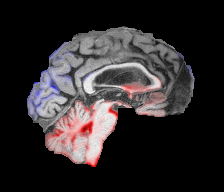
\includegraphics[height=2.5cm]{data/combined_sagittal.png}
            };

            \node[] at (0, 1) {
                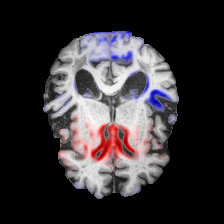
\includegraphics[height=2.5cm]{data/combined_axial.png}
            };

            \node[] at (3.25, 1) {
                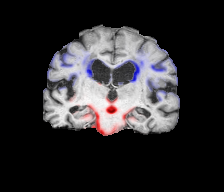
\includegraphics[height=2.5cm]{data/combined_coronal.png}
            };
            \node [
                left color=blue,
                right color=red,
                transform shape,
                draw=black,
                minimum height=0.25cm,
                text width=8cm,
            ] (colorbar) at (0, -1.5){};
            \node[font=\footnotesize\linespread{0.85}\selectfont, align=center, anchor=north] at (colorbar.south east) {
                Older\\appearing
            };
            \node[font=\footnotesize\linespread{0.85}\selectfont, align=center, anchor=north] at (colorbar.south west) {
                Younger\\appearing
            };
        }
        \visible<7>{
            \node[] at (0, 0) {
                \usebox{\patients}
            };
        }
        \visible<8>{
            \node[anchor=south] at (0, -3.5) {
                \usebox{\clinicalbaseline}
            };
        }\visible<9>{
            \node[anchor=south] at (0, -3.5) {
                \usebox{\clinicalbrainage}
            };
        }
        \visible<10>{
            \node[anchor=south] at (0, -3.5) {
                \usebox{\clinicalheatmaps}
            };
        }
    \end{tikzpicture}
\end{frame}


\end{document}
